% (c) 2002 Matthew Boedicker <mboedick@mboedick.org> (original author) http://mboedick.org
% 
% (c) 2011 Mite Mitreski <mitemitreski@gmail.com> http://mitemitreski.com
%


%This work is licensed under the Creative Commons Attribution-Noncommercial-Share Alike 2.5 License. To view a copy of this license, visit http://creativecommons.org/licenses/by-nc-sa/2.5/ or send a letter to Creative Commons, 543 Howard Street, 5th Floor, San Francisco, California, 94105, USA.

\documentclass[letterpaper,11pt]{article}

\newlength{\outerbordwidth}

\pagestyle{empty}

\raggedbottom

\raggedright

\usepackage[svgnames]{xcolor}

\usepackage[utf8]{inputenc}


\usepackage[english]{babel}
\usepackage[pdftex]{graphicx}


\usepackage{wrapfig}
\usepackage{framed}

\usepackage{tocloft}


\DeclareGraphicsExtensions{.pdf,.png,.jpg}

%-----------------------------------------------------------

%Edit these values as you see fit

\setlength{\outerbordwidth}{3pt}  % Width of border outside of title bars

\definecolor{shadecolor}{gray}{0.75}  % Outer background color of title bars (0 = black, 1 = white)

\definecolor{shadecolorB}{gray}{0.93}  % Inner background color of title bars

%-----------------------------------------------------------

%Margin setup

\setlength{\evensidemargin}{-0.25in}

\setlength{\headheight}{-0.25in}

\setlength{\headsep}{0in}

\setlength{\oddsidemargin}{-0.25in}

\setlength{\paperheight}{11in}

\setlength{\paperwidth}{8.5in}

\setlength{\tabcolsep}{0in}

\setlength{\textheight}{9.75in}

\setlength{\textwidth}{7in}

\setlength{\topmargin}{-0.3in}

\setlength{\topskip}{0in}

\setlength{\voffset}{0.1in}

%-----------------------------------------------------------

%Custom commands

\newcommand{\resitem}[1]{\item #1 \vspace{-2pt}}

\newcommand{\resheading}[1]{\vspace{8pt}

  \parbox{\textwidth}{\setlength{\FrameSep}{\outerbordwidth}

    \begin{shaded}

\setlength{\fboxsep}{0pt}\framebox[\textwidth][l]{\setlength{\fboxsep}{4pt}\fcolorbox{shadecolorB}{shadecolorB}{\textbf{\sffamily{\mbox{~}\makebox[6.762in][l]{\large #1} \vphantom{p\^{E}}}}}}

    \end{shaded}

  }\vspace{-5pt}

}

\newcommand{\ressubheading}[4]{
  \textbf{#1}  #2,
  \textit{#3}\\ \textit{#4}\\
}

%-----------------------------------------------------------

\begin{document}

 
\begin{tabular*}{7in}{l@{\extracolsep{\fill}}r}
 &  \raisebox{10pt}{ 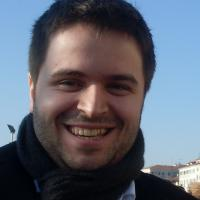
\includegraphics[scale=0.4]{me.jpg}} \\
\textbf{\Large Mite Mitreski} & \textbf{\today} \\
Software Engineer   & mite.mitreski@gmail.com \\
R.Novicic 74 Ohrid, Macedonia & blog.mitemitreski.com  \\
 & linkedin.com/in/mitemitreski \\

\end{tabular*}

%%%%%%%%%%%%%%%%%%%%%%%%%%%%%%

\resheading{Skills}

%%%%%%%%%%%%%%%%%%%%%%%%%%%%%%

\begin{itemize}

  \resitem {{\bf Software engineering}} \\ 
	 	Agile methodologies, Test Driven Development, Continuous Integration, Object-Oriented Design, Micro-service architecture, Domain Driven Design
  \resitem {{\bf Current technologies of choice include}} \\ 
	 	Java, JavaScript, Spring, Java EE, Node.js 
  \resitem{{\bf Regularly works with}}\\
	 	Bash, Zsh , Linux, HTML, Vim, Eclipse, Netbeans, Sublime Text, MySQL, Oracle
  \resitem {{\bf Has some work experience in}} \\ 
	 	 C\#, .NET, Pyhton2.x 
  \resitem {{\bf Knows the syntax of}} \\  
	 	C/C++, Lua, Clojure, CLisp, Pascal, BASIC, Processing, Prolog, Ruby, Python 

\end{itemize}
	

%%%%%%%%%%%%%%%%%%%%%%%%%%%%%%

\resheading{Work Experience}

%%%%%%%%%%%%%%%%%%%%%%%%%%%%%%

\begin{itemize}

\item []  
\ressubheading{Tricode}{Skopje, MK}{Software Engineer}{October 2013 - Present}
	\begin{itemize}
      \resitem{ Worked on a sales platform for LibertyGlobal containing  multiple countries and differt applications}
      \resitem{ Buissnes requirements and domain support}     
      \resitem{ Team leadership and professional growth}
      \resitem{ Technincal intreviewing and promotion }
      \resitem{ DevOps and change management of client services}
	\end{itemize}


\item []  
\ressubheading{Netcetera AG}{Skopje, MK}{Software Engineer}{August 2011 - October 2013}
	\begin{itemize}
      \resitem{ Work on domain specific solutions mostly for the financial sector in Switzerland}
      \resitem{ Work on Intranet integration software and customizations of Confluence}     
      \resitem{ Development of a common integration project for JavaScript build infrastructure into Java ecosystem}
      \resitem{ Mentioning of interns and new employees }
      \resitem{ DevOps and change management}
	\end{itemize}

\item []

	\ressubheading{Semos Edukacija }{Skopje, MK}{ Oracle Certified Java Trainer }{March 2010 - September 2012}

	\begin{itemize}
 
      \resitem{Fundamentals of the Java Programming Language, Java SE 6 (SL 110 SE6) }
      \resitem{Java Programming Language, Java SE 6 (SL 275 SE6) }
      \resitem{Developing Applications With the Java SE 6 Platform (SL 285 SE6)}
      \resitem{Developing Applications for the Java EE 6 Platform (FJ 310 EE6)}
      \resitem{Customized courses on topics related to Java EE}

	\end{itemize}
	
\item []

	\ressubheading{Faculty of electrical engineering and information technologies, FEIT }{Skopje, MK}{Lab assistant}{October 2010 - December 2010}

	\begin{itemize}
 
      \resitem{Teaching, creation of lab exercises, exam preparations }
     
	\end{itemize}

\item []

	\ressubheading{Genrepsoft}{Skopje, MK}{Software Development}{December 2007 - September 2010}

	\begin{itemize}
      
      \resitem{Development of debt management application for Ministry of Finance in Macedonia}
      \resitem{Development of custom Java EE/SE component based framework with custom markup}
      \resitem{Customization of Python based Q\&A clone of StackOverflow for USAID  }
    
	\end{itemize}
 
\item []

	\ressubheading{Other involvements}{Skopje, MK}{2006 - Present}{}

	\begin{itemize}
	  
	  \resitem{{\bf RoboMac 2010}, Organization, programming, fund-raising }
	  \resitem{{\bf RoboMac 2009}, Robotic competition co-founder, Organization, programming, fund-raising }
	  \resitem{{\bf Hacklab KIKA}, Participant in various programming related events}
 
	\end{itemize}
	
\end{itemize}

%%%%%%%%%%%%%%%%%%%%%%%%%%%%%%

\resheading{Volunteering}

%%%%%%%%%%%%%%%%%%%%%%%%%%%%%%
\begin{itemize}

  \item []
    \ressubheading{Java User Group Macedonia }{JUGMK}{Jug Leader}{December 2009 - Present}
   
    \begin{itemize}
      \resitem{Event organization, technical talks, management and fund-raising}
  	\end{itemize}

  \item []
    \ressubheading{IEEE Student Branch Macedonia }{}{Chairman, Secretary}{ 2007 - 2010}
   
    \begin{itemize}
      \resitem{Event organization, branch representation, book keeping, management and fund-raising}
  	\end{itemize}
 
\end{itemize}


%%%%%%%%%%%%%%%%%%%%%%%%%%%%%%

\resheading{Education}

%%%%%%%%%%%%%%%%%%%%%%%%%%%%%%

\begin{itemize}

\item []

	\ressubheading{Faculty of Electrical Engineering and Information Technologies}{Skopje, Macedonia}{Diploma degree, Informatics and computer engineering}{2006 - 2011}

	\begin{itemize}

		\resitem{National scholarship for talented students}
		\resitem{Diploma thesis: \textit{Automatic parallelization in compilers and parallel programming languages}}

	\end{itemize}
\item []
   \ressubheading{Sun certified Java programmer for SE 6}{April 2010}{}{}
 
\end{itemize}


%%%%%%%%%%%%%%%%%%%%%%%%%%%%%%

\resheading{Publications}

%%%%%%%%%%%%%%%%%%%%%%%%%%%%%%

\begin{itemize}
  \resitem{{\bf HTML5 Data and Services Cookbook, Packtpub , ISBN  978-1-78355-928-2}, co-author of a book about HTML5 and JavaScript }
\end{itemize}
 
\end{document}


